%Dies ist die Hauptseite des Dokumentes. Es werden u. a. alle Kapitel,
%Einstellung im Header eingebunden.  Veränderungen müssen in folgenden Dateien
%vorgenommen werden:
      %- Layout.tex
      %- newComments.tex
      %- Titelseite
      %- Versionsübersicht
      %- einzelne Kapitel (evtl. erweitern)


% Definition von globalen Parametern, die derzeit auf der Titelseite und in der
% Kopfzeile verwendet werden. Der in <> gesetzte Text ist zu verändern.

\newcommand{\praktikumTitel}{Ingenieursmäßige Konstruktion, Simulation und Visualisierung von Achterbahnen }
\newcommand{\projektTitel}{Achterbahnsimulator}


%Hier sind alle Einstellungen enthalten, die sich auf das Seiten- und
%Dokumentenlayout beziehen

\documentclass[
  11pt,                % Schriftgröße
  DIV12,
  german,              % für Umlaute, Silbentrennung etc.
  oneside,             % einseitiges Dokument
  titlepage,           % es wird eine Titelseite verwendet
  halfparskip,         % Abstand zwischen Absätzen (halbe Zeile)
  normalheadings,      % Größe der Überschriften verkleinern
  tablecaptionabove,   % Beschriftung von Tabellen unterhalb ausgeben
  final                % Status des Dokuments (final/draft)
]{scrreprt}            %


%------Ändern von Schriftschnitten - (Muss ganz am Anfang stehen !) ------------
\usepackage{fix-cm}

%------Umlaute -----------------------------------------------------------------
%   Umlaute/Sonderzeichen wie äüöß können direkt im Quelltext verwenden werden.
%    Erlaubt automatische Trennung von Worten mit Umlauten.
\usepackage[T1]{fontenc}
\usepackage[utf8]{inputenc}

%------Anpassung der Landessprache----------------------------------------------
\usepackage{ngerman}

%------Einfache Definition der Zeilenabstände und Seitenränder------------------
\usepackage{geometry}
\usepackage{setspace}

%------Schriftgrößenanpassung von einzelnen Textpassagen------------------------
\usepackage{relsize}

%------Trennlinien in Kopf- und Fusszeile
\usepackage[headsepline, footsepline, ilines]{scrpage2}

%------Grafiken-----------------------------------------------------------------
\usepackage{graphicx}

%------Packet zum Sperren, Unterstreichen und Hervorheben von Texten------------
\usepackage{soul}

%------ergänzende Schriftart----------------------------------------------------
\usepackage{helvet}

%------Lange Tabellen-----------------------------------------------------------
\usepackage{longtable}
\usepackage{array}
\usepackage{ragged2e}
\usepackage{lscape}

%------PDF-Optionen-------------------------------------------------------------
\usepackage[
  bookmarks,
  bookmarksopen=true,
  colorlinks=true,
  linkcolor=black,        % einfache interne Verknüpfungen
  anchorcolor=black,      % Ankertext
  citecolor=black,        % Verweise auf Literaturverzeichniseinträge im Text
  filecolor=black,        % Verknüpfungen, die lokale Dateien öffnen
  menucolor=black,        % Acrobat-Menüpunkte
  urlcolor=black,         % Farbe für URL-Links
  backref,                % Zurücktext nach jedem Bibliografie-Eintrag als
                          % Liste von Überschriftsnummern
  pagebackref,            % Zurücktext nach jedem Bibliografie-Eintrag als
                          % Liste von Seitenzahlen
  plainpages=false,       % zur korrekten Erstellung der Bookmarks
  pdfpagelabels,          % zur korrekten Erstellung der Bookmarks
  hypertexnames=false,    % zur korrekten Erstellung der Bookmarks
  linktocpage             % Seitenzahlen anstatt Text im Inhaltsverzeichnis
                          % verlinken
  ]{hyperref}



      % enthält eingebundene Packete

%------Seitenränder-------------------------------------------------------------
\geometry{verbose,                     % zeigt die eingestellten Parameter beim
                                       % Latexlauf an
      paper=a4paper,                   % Papierformat
      top=25mm,                        % Rand oben
      left=25mm,                       % Rand links
      right=25mm,                      % Rand rechts
      bottom=45mm,                     % Rand unten
      pdftex                           % schreibt das Papierformat in die
                                       % Ausgabe damit Ausgabeprogramm
                                       % Papiergröße erkennt
  }

%Seitenlayout
\onehalfspace        % 1,5-facher Abstand

%------Kopf- und Fußzeilen -----------------------------------------------------
\pagestyle{scrheadings}

%------Kopf- und Fußzeile auch auf Kapitelanfangsseiten ------------------------
\renewcommand*{\chapterpagestyle}{scrheadings}

%------Schriftform der Kopfzeile -----------------------------------------------
\renewcommand{\headfont}{\normalfont}

%------Kopfzeile----------------------------------------------------------------
\setlength{\headheight}{21mm}        % Höhe der Kopfzeile
\ihead{\large{\textsc{\praktikumTitel}}\\    % Text in der linken Box
       \small{\projektTitel}}
\chead{}                             % Text in der mittleren Box

%----Fusszeile
\cfoot{}                             % Text in mittlerer Box
\ofoot{\pagemark}                    % Seitenzahl in rechter Box

          % Diese Datei enthält alle
                                          % Layouteinstellungen

%------Beginn des Gesamtdokumentes----------------------------------------------
\begin{document}

%------Eingebundene Seiten, Verzeichnisse bzw. Kapitel--------------------------
% Dies ist die Titelseite des Pflichtenhefts.
% Die in "<...>" sind zu ersetzen
% Die Ausgabe darf 1 Seite nicht überschreiten, also ggf. Abstände anpassen
% Die Angabe in [...] gibt den Abstand nach der entsprechenden Zeile an.


%----Stil dieser Seite----------------------------------------------------------
\thispagestyle{plain}      % Kopfzeile bleibt leer

%----Beginn der Titelseite------------------------------------------------------
\begin{titlepage}

%----zentrierte Ausrichtung über die gesamte Seite----------------------------
\begin{center}

%----Titel des Praktikum (\praktikumTitel in newComments zu verändern)--------
{\relsize{4}{\textbf{\textsc{\praktikumTitel}}}}\\[5ex]

%----Titel des Teilprojektes (\projektTitel in newComments verändern)---------
{\relsize{3}{\textbf{\textsc{\projektTitel}}}}\\[5ex]

Software-Entwicklungspraktikum (SEP)\\
Sommersemester 2011\\[6ex]

{\relsize{3}\so{\textbf{Pflichtenheft}}}\\[5ex]

%----eingebundenes Logo der TU--------------------------------------------------

\includegraphics[scale=0.8]{bilder/carolo.jpg}\\[5ex]

%----Daten des Auftraggebers
Auftraggeber\\
Technische Universität Braunschweig\\
Institut für Wissenschaftliches Rechnen\\
Prof. Hermann G. Matthies, PhD\\
<Straße und Hausnummer>\\
D-38092 Braunschweig\\[2ex]
Betreuer: Elmar Zander\\[5ex]

% ----Tabelle der Praktikumsteilnehmer------------------------------------------
Auftragnehmer: <überzählige Zeilen löschen>\\

\begin{tabular}{l<{\hspace{20mm}} l<{\hspace{30mm}}}\\
  Name                   &   E-Mail-Adresse\\      % Zeilenüberschift

  \hline                    % Linie unterhalb der Zeilenüberschrift

  %----Nachfolgend alle Namen und E-Mail-Adressen der Teilnehmer einfügen
  Matthias Überheide> &  m.ueberheide@tu-bs.de\\
  Christian Mangelsdorf &  ch.mangelsdorf@googlemail.com\\
	Daniel Bahn & danielbahn@arcor.de\\
	Simon Hahne & MrSimWob@aol.com\\
	Robin Hofmann & hofmann.robin@web.de\\
	Marco Melzer & marco.melzer@tu-braunschweig.de\\
	Konstantin Birker & k.birker@tu-braunscheig.de\\

\end{tabular}\\[2ex]

Braunschweig, \today

\end{center}
\end{titlepage}
                      % Titelseite

%Diese Datei dient der Versionskontrolle. Sie ist vollständig zu bearbeiten.

%----Überschrift------------------------------------------------------------
{\relsize{2}\textbf{Versionsübersicht}}\\[2ex]

%----Start der Tabelle------------------------------------------------------
\begin{longtable}{|m{1.78cm}|m{1.59cm}|m{2.86cm}|m{1.9cm}|m{5.25cm}|}

  \hline                                              % Linie oberhalb

  %----Spaltenüberschriften------------------------------------------------
  \textbf{Version}  &    \textbf{Datum}  &    \textbf{Autor}  &
  \textbf{Status}   &    \textbf{Kommentar}       \\  %Spaltenüberschrift
  \hline                                              % Gitterlinie

  %----die nachfolgeden beiden Zeilen so oft wiederholen und die ... mit den
  %    entsprechenden Daten zu füllen wie erforderlich
  0.1&02.05.2011&Christian Mangelsdorf&in Bearbeitung&Initialisierung\\
  \hline
  0.2&04.05.2011&Simon Hahne, Robin Hoffman, Christian Mangelsdorf&in Bearbeitung&Komponentenspezifiktion\\
  \hline
  0.3&06.05.2011&Matthias Überheide&in Bearbeitung&Vorbereitung Funktionsanalyse\\
  \hline
  0.4&08.05.2011&Matthias Überheide, Daniel Bahn, Konstantin Birker, Robin Hoffman, Simon Hahne, Christian Mangelsdorf&in Bearbeitung&Sequenzdiagramme und Statcharts\\
  \hline
  0.5&09.05.2011&Matthias Überheide, Daniel Bahn, Robin Hoffman, Simon Hahne, Christian Mangelsdorf&in Bearbeitung&Änderungen gemäß Besprechung\\
  \hline
  0.6&10.05.2011&Matthias Überheide, Christian Mangelsdorf&in Bearbeitung&Schnittstellenspezifikation\\
  \hline
  0.7&11.05.2011&Matthias Überheide, Daniel Bahn, Konstantin Birker, Robin Hoffman, Simon Hahne, Christian Mangelsdorf, Marco Melzzer&abgenommen&Korrekturen\\
  \hline
  %...    &    ...    &    ...    &    ...    &    ...\\       % Eintrag in Zeile
  \hline                                              % Gitterlinie unten

%----Ende der Tabelle------------------------------------------------------
\end{longtable}

%Status: "`in Bearbeitung"' oder "`abgenommen"'
%Kommentar: hier eintragen, was geändert bzw. ergänzt wurde


%Hinweis zum Template:
%Dieses Template enthält Hinweise, die alle kursiv geschrieben sind. Alles
%Kursivgeschriebene ist selbstverständlich bei Abgabe zu entfernen sind.
%Angaben in <\ldots> sind mit dem entsprechendem Text zu füllen.  Überzählige
%Kapitel, d. h. Kapitel, die nicht bearbeitet werden müssen, da sie nicht der
%Aufgabenstellung entsprechen, bitte entfernen.

%Aufgabe des Grobentwurfs: Aufgabe dieses Dokumentes ist es, die Architektur des
%Systems zu beschreiben und die daraus resultierenden Pakete durch die
%Definition von Schnittstellen zu Komponenten auszubauen.
       % Versionsübersicht

\tableofcontents                          % Inhaltsverzeichnis wird automatisch
                                          % generiert
\listoffigures                            % ebenso das Abbildungsverzeichnis

%Abbildung 1: StateChart Projektdetails  5 \\
%Abbildung 2: Verteilung von <ID>  7       \\
%Abbildung 3: Sequenzdiagramm für <ID>  7  \\
%Abbildung 4: Komponentendiagramm  8       \\
%Abbildung 5: Protokollstatechart für jede Komponente  9    \\
%Abbildung 6: Verteilungsdiagramm  10      \\




%----Kapitel des Feinentwurfs, die mit Inhalt zu füllen sind--------------------
% Kapitel 1
% Die Unterkapitel können auch in separaten Dateien stehen,
% die dann mit dem \include-Befehl eingebunden werden.
%-------------------------------------------------------------------------------

\chapter{Einleitung}
%Hier Einleitungstext einfügen, dabei die Formatierungen selber erstellen
%Hier ist die Arbeitsweise des Systems anhand von State-Charts darzustellen und kurz zu erläutern.

Die Anwendung ist ein Werkzeug zur physikalischen Simulation und 3D-Visualisierung von Achterbahnfahrten.
Der Benutzer wählt dazu eine Datei mit der Spezifikation des Streckenverlaufes aus. Die Anwendung erstellt 
daraus ein virtuelles Modell der Achterbahn und simuliert physikalisch korrekt die Bewegung des Wagens mit
der Zeit. In den folgenden Abschnitten wird Arbeitsweise des Simulators detailiert.

\section{Projektdetails}
Die Funktionalität der Anwendung gliedert sich in mehrere zusammenhängende Teilbereiche. Jeder dieser
Bereiche bündelt eine Reihe der Anforderungen, die im Pflichtenheft spezifiziert worden sind.

\subsection{Benutzeroberfläche}
Über die Benutzeroberfläche (GUI) werden dem Anwender alle vorhandenen Funktionen zugänglich gemacht.
Nach dem Programmstart befindet sich der Anwender in einem Initialzustand: Die Felder des 2D-Modells
und der 3D-Darstellung befinden sich in einem Blanko-Zustand und die physikalischen Parameter sind
auf die Standardwerte gesetzt. Der nächte Schritt ist die Auswahl einer Datei mit den Konstruktionsdaten
über ein Dateimenü. Nach dem Einlesen der Datei zeigt die Anwendung zunächst eine zweidimensionale 
Vorschau der Achterbahn an. Zu diesem Zeitpunkt können über ein Optionen-Menü verschiedene Anpassungen 
an den Grafikeinstellungen und den physikalischen Parameter vorgenommen werden. 
Aus der Vorschau heraus kann die Simulation gestartet werden. Ab diesem Zeitpunkt wird das Feld für 
die 3D-Darstellung befüllt. Auf Wunsch kann die 3D-Darstellung auf Bildschirmgröße
maximiert werden. Während der laufenden Simulation können die Grafikeinstellungen, nicht jedoch
die physikalischen Simulationsparameter angepasst werden. Wird die Simulation gestoppt, kehrt die Anwendung
wieder in die Vorschau zurück. Durch Schließen der Achterbahndatei gelangt der Benutzer wieder in den 
Initialzustand.

\begin{figure}
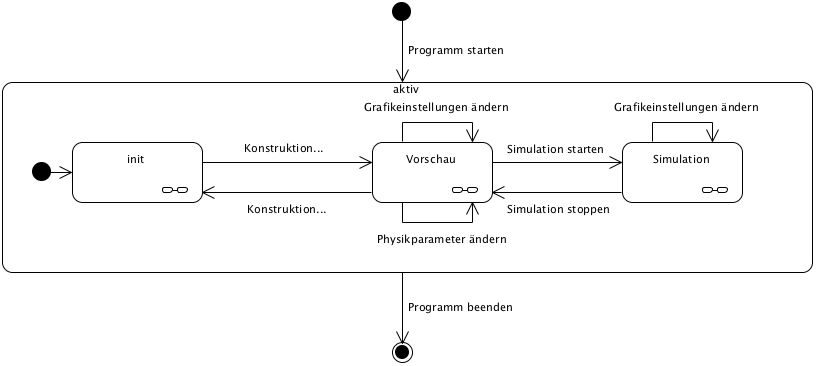
\includegraphics[width=\linewidth]{bilder/StateChart_GUI}
\caption{Statechart für die \textit{Benutzeroberfläche}}
\end{figure}

\subsection{Simulator}
Der Simulator ist das Kernstück der Anwendung und repräsentiert das Zusammenspiel aus physikalischen Berechnungen
und grafischer Darstellung der Achterbahnfahrt. Die Zustandswechsel des Simulators verlaufen synchron mit 
denen der Benutzeroberfläche. Nach dem Starten des Programms befindet sich der Simulator in einem Initialzustand,
der noch keine Simulation repräsentiert. Durch das Befüllen mit der Spezifikation der Achterbahn wird
eine Simulation instanziert und zur Vorschau gebracht. Mit dem Start der Simulation werden in diskreten Zeitschritten
die aktualisierten physikalischen Daten eingelesen und zur Veränderung der Kameraposition verwendet. Durch das
Stoppen der Simulation kehrt auch der Simulator wieder in die Vorschau zurück.

\subsection{3D-Anzeige}
Die 3D-Anzeige dient zur Visualisierung der Achterbahnfahrt, also zur Darstellung der Bahn als 3D-Modell aus
einer vorgegebenen Kameraperspektive. Vor der Bereitstellung eines konkreten Achterbahnmodells befindet sich
die Anzeige in einem Initialzustand, in welchem es in Ermangelung von Daten nicht möglich eine Szene darzustellen. 

\begin{figure}
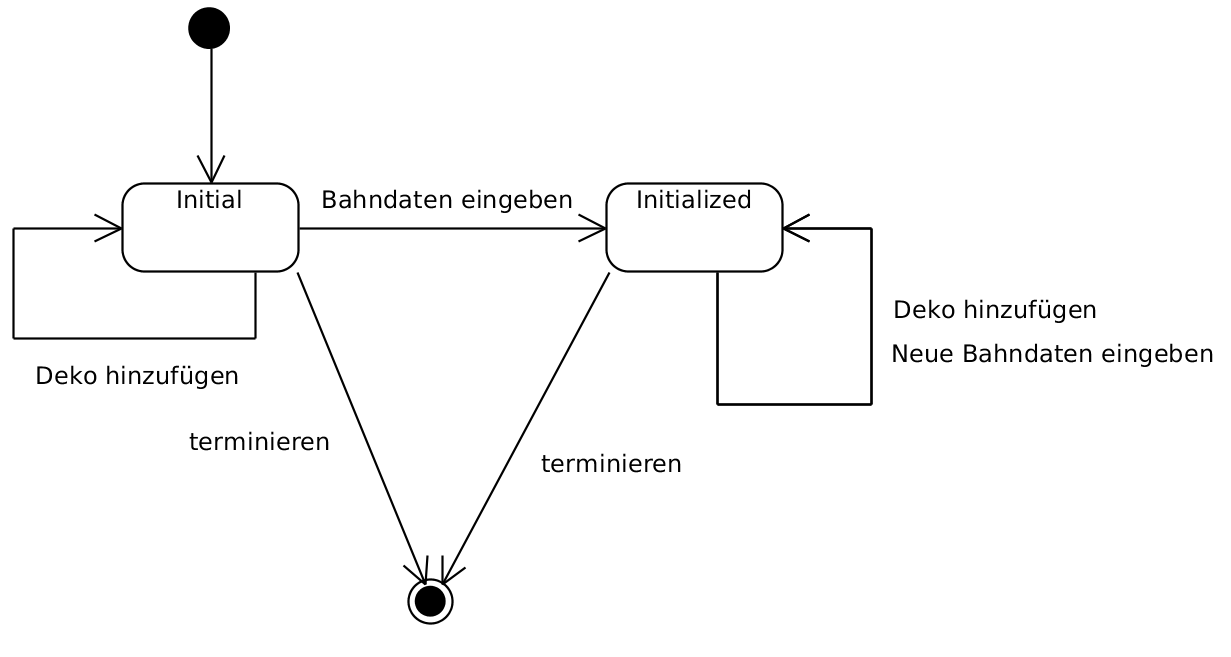
\includegraphics[width=\linewidth]{bilder/statechart_3dgraphics}
\caption{Statechart für die \textit{3D-Anzeige}}
\end{figure}

Durch Übergabe der Bahndaten kann die 3D-Anzeige die Achterbahn und deren Umgebung für die Anzeige vorberechnen.
Aber erst nach dem Start der Simulation, werden regelmäßig Bilder berechnet und angezeigt. Aus Sicht der 3D-Anzeige
können nach der Beladung jederzeit Änderungen wie Einfügen von Dekoration oder Anpassen der grafischen Einstellungen
vorgenommen werden, ohne das eine Zustandsänderung erforderlich wäre. Allerdings müssen innerhalb des Render-Vorgangs
eines einzelnen Bildes die Einstellungen unverändert bleiben, damit eine saubere Kommunikation mit dem 3D-Hardwarekontext
gewahrt bleibt.

\subsection{Physik und Mathematik}

Die physikalischen Berechnungen des Achterbahnsimulators folgen den Gesetzen der Newtonschen Mechanik für die Bewegung
eines Massenpunktes auf einer vorgegebenen Bahn im Gravitationsfeld der Erde. Berechnet wird die Bahnkurve als Lösung
einer gewöhnlichen Differentialgleichung mit vorgegebenen Anfangswerten. Die Lösung erfolgt nach einem numerischen
Verfahren, welches über die Zeit integriert.

Entsprechend wird der Zustand des Systems nach der Initialisierung mit den Bahndaten und den Anfangswerten von Zeitpunkt
zur Zeitpunkt weiterentwickelt, bis die Simulation (z.B. über Programmende) beendt wird.

Für die Berechnung der Bahnkurven kommen eine Reihe von Hilfsmethoden zum Einsatz. Diese Routinen sind zustandslos und
besitzen keinen eigenen Lebenszyklus.

\begin{figure}
\includegraphics[width=\linewidth]{bilder/statechart_physics}
\caption{Statechart für die \textit{Physik}}
\end{figure}
                % Kapitel 1
% Kapitel 2 mit den entsprechenden Unterkapiteln
% Die Unterkapitel können auch in separaten Dateien stehen,
% die dann mit dem \include-Befehl eingebunden werden.
%-------------------------------------------------------------------------------
\chapter{Analyse der Produktfunktionen}

Dieser Abschnitt stellt die Basis für die Festlegung der Architektur dar. Die
Festlegung einer geeigneten Architektur geschieht aufgrund der im Pflichtenheft
analysierten Produktfunktionen und nicht-funktionalen Anforderungen, die
realisiert werden müssen. Jede betrachtete Funktion wird in einem eigenen
Unterkapitel dokumentiert.  Fügen Sie bitte so viele Unterkapitel ein, wie
Produktfunktionen im Pflichtenheft vorhanden sind. Auch die nicht-funktionalen
Anforderungen sind so weit möglich entsprechend darzustellen.

%Die Kapitel müssen mit Inhalt gefüllt werden!. Eine Bereiche habe ich beuwsst schon bei der Verteildung der Diagramme zusammengefasst 
%In diesen Bereichen möchte ich euch bitten die jeweiligen Unterpunkte kurz mit den Oberpunkten zu vergleichen und zu argumentieren 
%warum es sich um triviale Spezialfälle handelt die keiner näheren beschreibung bedürfen
%
% Ich hab mal immer davon geschrieben welche Bereich von wem gemacht werden





%Christian/Matthias

%kann man dies ggf Q40 zuordnen?
\section{Analyse von Funktionalität :  Renderloop}
Da es sich um ein System handelt, indem eine ständige Berechnung (Loop) zur Laufzeit notwendig wird, einerseits durch die 3D-Anzeige die eine ständige aktualisierung erwartet und andererseits durch
die Simulation an sich, ist es sinnig diesen Vorgang ebenfalls näher zu beleuchten.
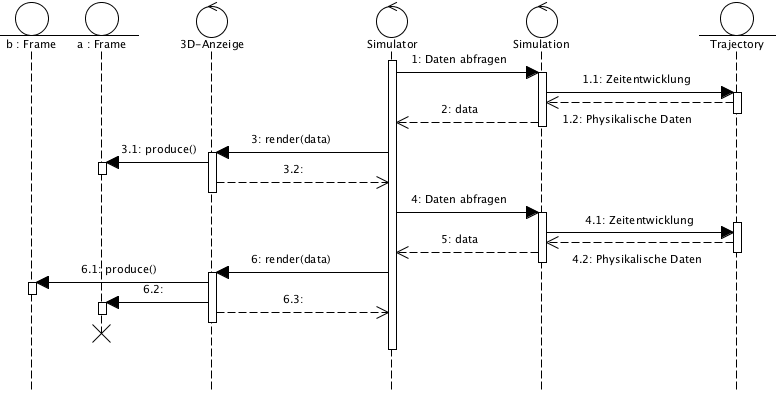
\includegraphics[width=16cm]{bilder/render_loop}

%Marco:
\section{Analyse von Funktionalität /F100/ :  Spezifikation einlesen }
%Simon:
\section{Analyse von Funktionalität /F200/ :  Starten/Stoppen der Simulation}
%Robin
\section{Analyse von Funktionalität /F300/ :  Pausieren der Simulation}
%Daniel
\section{Analyse von Funktionalität /F400o/ :  Video aufzeichnen}
%Matthias/Christian
\section{Analyse von Funktionalität /F500/ :  Einstellungen ändern}
\subsection{Analyse von Funktionalität /F510o/ :  Physikalische Paramter anpassen}
% Hier reicht ein Sequenzdiagramm, das zeigt das Änderungen an den physikalischen Paramtern das stoppen der Simulation zur Folge haben
% die folgenden Kapitel würde ich daher in einem zusätzlichen Textkommentar zusammenfassen
\subsubsection{Analyse von Funktionalität /F511o/ :  Gravitation anpassen}
\subsubsection{Analyse von Funktionalität /F512o/ :  Wagenmasse anpassen}
%Matthias
\subsection{Analyse von Funktionalität /F520/ :  Simulationsparameter ändern}
Die Veränderung von Parametern die die Simulation direkt betreffen fallen unter diese Oberklasse. Die einzelnen Unterpunkte werden in den 2 folgenden Kapiteln erläutert. Im wesentlichen Fallen hier 
auch einfache Veränderungen an, die als atomistisch und somit unkritisch anzusehen sind. In der Folge werden diese Use-Cases nicht extra in Sequenzdiagrammen abgebildet.
\subsubsection{Analyse von Funktionalität /F521o/ :  Dekorative Umgebung anpassen}
Da diese Aktion in den Datenbestand des 3D-Kontext eingreift gibt es einen interessanten Fall in dem das direkte Setzen der Deko nicht möglich ist. 
Der User fordert die Veränderung der Deko über die 2D-GUI an (2). Kurz zuvor wurde aber das Render eine Frames(1) angefordert. In der Folge muss die 3D Anzeige mit der Veränderung der Konfiguration (1.3)
bis zum Abschluss des Rendervorgangs (1.2) warten. Dann kann die Deko gemäß der Uservorgaben geladen werden(1.4). In (1.5) meldet sich die 3D-Anzeige bei den anderen Komponenten zurück. 

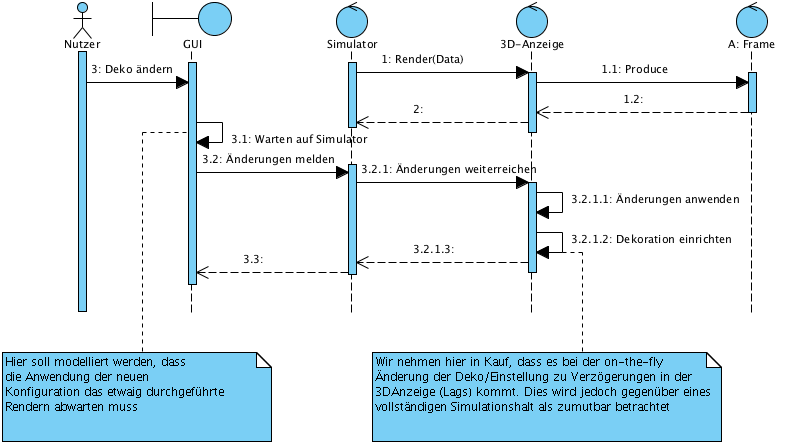
\includegraphics[width=16cm]{bilder/change_graphic_deko}

Es wird hier in Kauf genommen, dass die Simulation für eine spürbare Zeit unterbrochen wird um die Deko zu laden. Dies wird als zumutbar angenommen um undefinierte Zustände zu verhindern. 
Außerdem wird erwartet, dass die Funktionalität selten während der laufenden Simulation sondern vor dem Start genutzt wird wo auch Wartezeiten akzeptabel sind.

\subsubsection{Analyse von Funktionalität /F522o/ :  Simulatioszeit anpassen}
Die Simulationsgeschwindigkeit wird, aufgrund der Implementierung eines numerischen Lösungsverfahrens für die Berechnung der Daten ein diskreter Zeitschritt sein. Dieser Wert kann direkt und entsprechend
den Anforderungen des Nutzers gesetzt werden. Das einfache Durchreichen über die GUI an den Simulator wird nicht in einem zusätzlichen Sequenzdiagramm dargestellt.
%Matthias
\subsection{Analyse von Funktionalität /F530/ :  Graphische Einstellungen ändern}
Die Anpassung der grafischen Einstellung bezieht sich hier zunächst allgemein auf graphische Einstellungen. Besonders interessant ist dabei jedoch der Fall der Veränderung von Einstellungen die 
die 3D-Anzeige betreffen. 

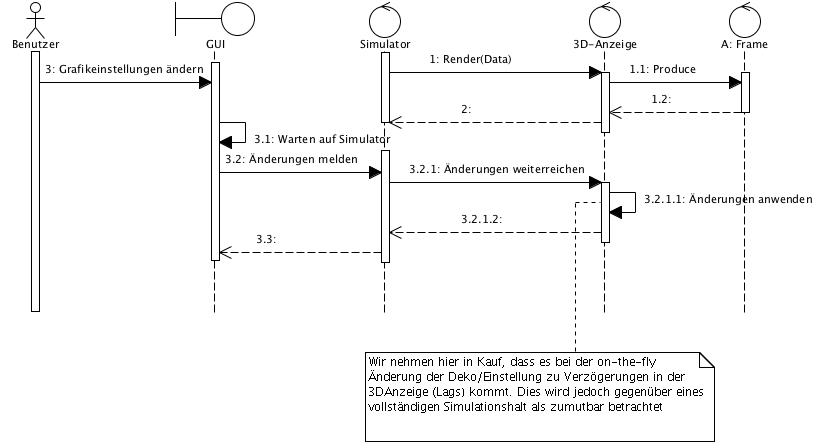
\includegraphics[width=16cm]{bilder/change_graphic_config}

Fordert der Nutzer die Veränderung von Einstellungen aus dem 3D-Kontext an (2), so besteht die Möglichkeit, dass zum gleichen Zeitpunkt ein Frame, initiiert durch den Simulator (1), gerendert wird. 
Die GUI (hier für den 2D-Anteil) wird die Anfrage des Benutzer an die 3D-komponente weiterreichen(2.1) und eine etwaige Bestätigung (beispielsweise durch Statusveränderung des Konfigurationsdialogs) an den 
User ausgeben (2.2). Die 3D-Komponente muss jetzt den Renderprozess abwarten und darf erst dann die veränderte Konfiguration anwenden um ungültige Zustände zu vermeiden. Die Anwendung der Konfiguration verzögert 
die Rückmeldung der Bereitschaft an den Simulator(2.1.4) um sicherzustellen, dass nicht mit einem neuen Frame begonnen wird bevor die Einstellungen übernommen wurden. 

Bei diesem Vorgehen wird in Kauf genommen, dass es für das Frame was auf die Einstellungsänderung folgt zu einer Verzögerung in der Darstellung kommt. Dies muss jedoch als zumutbar erachtet werden, da zum einen
eine Zeitdauer im Millisekundenbereich zu erwartet ist. Die Alternativen beinhalten wesentlich störendere Artefakte oder aber das grundsätzliche Anhalten der Simulation nach Änderungen an den Einstellungen.

%Daniel
\subsubsection{Analyse von Funktionalität /F531/ :   Neuanordnung (Interface)}
%Simon
\subsubsection{Analyse von Funktionalität /F532/ :  Ein-/Ausblenden von Beschleunigungsdaten}
%Robin
\subsubsection{Analyse von Funktionalität /F533o/ :  Kameraperspektive ändern}
%Konstantin
\section{Analyse von Funktionalität /F1000/ :  Warnung vor hoher Beschleunigung}
%Marco:
\section{Analyse von Funktionalität /F1100/ :  Erkennung von Veränderungen an der Ursprungsdatei}  % Kapitel 2
% Kapitel 3 mit den entsprechenden Unterkapiteln
% Die Unterkapitel können auch in separaten Dateien stehen,
% die dann mit dem \include-Befehl eingebunden werden.
%------------------------------------------------------------------------------------
\chapter{Resultierende Softwarearchitektur}

Dieses Kapitel erläutert die geplante Architektur des Achterbahnsimulators und
liefert eine grobe Spezifikation der Schnittstellen zwischen den geplanten
Komponenten.

\section{Komponentenspezifikation}

Aus der Analyse der Produktfunktionen ergeben sich sechs größere Teilbereiche,
die als Komponenten dieser Anwendung umgesetzt werden soll.

Im Kern der Anwendung steht die Simulator-Komponente, die für die Steuerung der
Achterbahnbewegung verantwortlich ist und zwischen der physikalischen Berechnung
und der grafischen Umsetzung koordiniert. Dieser Komponente wird von Außen die
Spezifikation einer Achterbahn übergeben, welche als Simulation umgesetzt werden
soll. Die Komponente hält über eine Endlosschleife (``render loop'') den Ablauf im Gang.

Die dreidimensionale Visualisierung der Achterbahn mit Gerüst und Umgebung wird
von der 3D-Anzeige-Komponente (``3D Graphics Engine'') übernommen. Sie kapselt die allgemeinen gehaltenen
Funktionen der eingesetzten Grafikbibliothek und stellt eine einfache Schnittstelle
für das Befüllen der virtuellen Welt mit Achterbahnkomponenten sowie zur Steuerung
der Kamerafahrten entlang der befahrenen Strecke zur Verfügung.

Die physikalische Berechnung der Achterbahnbewegung erfolgt in der Physik-Komponente
(``Physics'' Engine). Hier wird die Bewegung eines Massenpunktes auf der vorgegebenen Raumkurve
nach den Gesetzen der klassischen Mechanik durch Lösen einer gewöhnlichen 
Differentialgleichung bestimmt. Die berechnete Bahnkurve wird dem Simulator zur
Umsetzung der Kamerafahrt bereitgestellt.

Um die über Stützstellen definierte Achterbahn in eine ununterbrochene und hinreichend
glatte Raumkurve umzurechnen, kommt die Mathematik-Komponente (``Mathematics'') zum Einsatz. Im
Wesentlichen besteht die Komponente aus den Routinen zur näherungsweisen Berechnung
von Beziérkurven. 

Für das Einlesen der Achterbahn-Spezifikationen aus den vom Editor bereitgestellten
XML-Dateien kommt die Dateiverwaltungs-Komponente (``File Management'') zum Einsatz. Diese kapselt alle
am speziellen Serialisierung-Schema haftenden Eigenheiten ab und liefert einen
von den anderen Komponenten einfach auslesbaren Datensatz mit dem Stützstellen der
Bahn und weiteren Parametern.

Die grafische Benutzeroberfläche (``Graphical User Interface'') übernimmt die Interaktion zwischen dem Benutzer und
der Simulation. Es übernimmt die Steuerung des Hauptmenüs, des Dateidialoges und
des Optionen-Dialogs. Die aus der Dateiverwaltung ausgelesenen Achterbahn-Datensätze 
werden an den Simulator zur Darstellung übergeben. Die Nutzeraktionen bezüglich des
Simulationsablaufes werden durchgereicht.

\begin{figure}
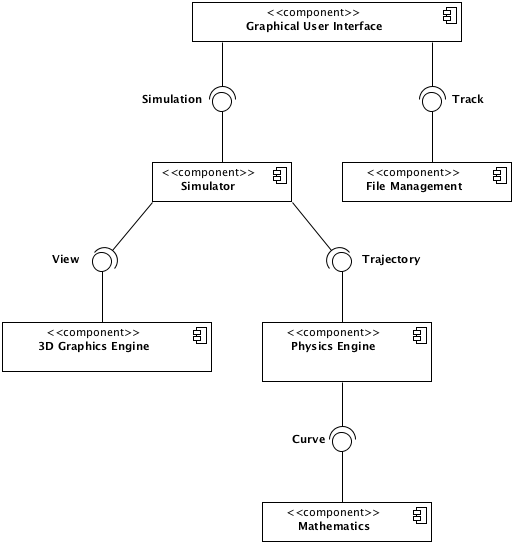
\includegraphics[width=\linewidth]{bilder/component_overview}
\caption{Komponentendiagramm für den Achterbahnsimulator}
\label{labelname}
\end{figure}

\section{Schnittstellenspezifikation}

Im Folgenden werden die einzelnen Schnittstellen der Komponenten aus der
Komponentenspezifikation näher erläutert, d. h. die von ihnen zur Verfügung
gestellten Operationen werden dokumentiert. Die Tabelle ist dabei um so viele
Zeilen zu erweitern, wie es Schnittstellen im Komponentendiagramm gibt. In der
innen liegenden Aufteilung ist für jede Operation einer Schnittstelle eine
Zeile einzufügen.  Reine Set- und Get-Aufrufe brauchen nicht aufgeführt zu
werden (sollten auch möglichst nicht komponentenübergreifend auftauchen).

\begin{tabular}[ht]{|l|p{0.35\linewidth}|p{0.35\linewidth}|}
 \hline
 Schnittstelle & \multicolumn{2}{|c|}{Aufgabenbeschreibung}\\
 \hline
 \hline
    /S10/ Track & \multicolumn{2}{|c|}{Spezifikation der Achterbahn mit Stützstellen und Parametern}\\
 \hline
 & getCurve() : Curve & Liefert die Achterbahnstrecke als mathematische Raumkurve zurück.\\ 
 \hline
    /S20/ Curve & \multicolumn{2}{|c|}{Repräsentation einer ortientierten Raumkurve}\\
 \hline
 & getLength() : double & Liefert die Länge der Raumkurve.\\ 
 & getPoint(lengh : double) : CurvePoint & Liefert den Repräsentanten für einen bestimmen Punkt auf der Raumkurve zurück,
 wobei über die Bogenlänge parametrisiert wird.\\ 
 & getPointSequence(maxDistance : double, maxAngle : double) : List<CurvePoint> &
 	Liefert eine Liste mit Punkten auf der Raumkurve wieder, die höchsten den angegebenen Abstand und die
 	Differenz im Raumwinkel haben dürfen. \\
 \hline
    /S21/ CurvePoint & \multicolumn{2}{|c|}{Repräsentation eines bestimmten Punktes auf einer Raumkurve}\\
 \hline
 & getPosition() : Vector & Liefert die Position. \\
 & getRollAxis() : Vector & Liefert die Rollachse (Längsachse).\\ 
 & getPitchAxis() : Vector & Liefert die Nickachse (Querachse). \\ 
 & getYawAxis() : Vector & Liefert die Gierachse (Hochachse). \\
 \hline
 	/S30/ Trajectory & \multicolumn{2}{|c|}{Bahnkurve einer Punktmasse als Funktion der Zeit}\\
 \hline
 & getCurve() : Curve & Liefert den räumlichen Verlauf der Bahnkurve als Raumkurve zurück.\\ 
 & getPoint(time : double) : TrajectoryPoint & Liefert den Repräsentanten für einen bestimmten Punkt auf der Bahnkurve zurück.\\ 
 %& Name der Funktion3 & Beschreibung3\\ 
 %& Name der Funktion4 & Beschreibung4\\ 
 \hline
 	/S31/ TrajectoryPoint & \multicolumn{2}{|c|}{Repräsentation eines bestimmten Punktes auf der Bahnkurve}\\
 \hline
 & getPosition() : Vector & Liefert die momentane Position.\\ 
 & getVelocity() : Vector & Liefert die m. Geschwindigkeit.\\ 
 & getAcceleration() : Vector & Liefert die m. Beschleunigung. \\ 
 \hline
 \end{tabular}

\begin{tabular}[ht]{|l|p{0.35\linewidth}|p{0.35\linewidth}|}
 \hline
 Schnittstelle & \multicolumn{2}{|c|}{Aufgabenbeschreibung}\\
 \hline
 \hline
    /S40/ Simulation & \multicolumn{2}{|c|}{Repräsentant für eine konkrete Simulation}\\
 \hline
 & start() : void & Startet die Simulation.\\ 
 & stop() : void & Stoppt die Simulation. \\ 
\hline
	/S50/ View & \multicolumn{2}{|c|}{Repräsentant für die 3D-Welt mit bestimmter Kameraperspektive}\\
\hline
 & setCamera(positon : Vector, direction : Vector) & Setzt die Kamera auf die angegebene Position und Raumrichtung. \\ 
 \hline

 & setCurve(curve : Curve) & Setzt die Bahndaten die zur Darstellung kommen sollen. \\ 
 \hline

 \end{tabular}





\section{Protokolle für die Benutzung der Komponenten}

%In diesem Abschnitt wird mit Hilfe von Protokoll-Statecharts die korrekte
%Verwendung der zu entwickelnden Komponenten dokumentiert. Dies ist insbesondere
%für diejenigen Komponenten notwendig, für die eine Wiederverwendung möglich
%erscheint oder sogar bereits geplant ist.

%Begründen Sie für welche Komponenten eine Wiederverwendung sinnvoll erscheint
%und für welche nicht!
Der Achterbahnsimulator setzt trotz seines (schon durch den Namen ersichtlichen)
eingeschränkten Anwendungsbereiches bereits alle wesentlichen Teile für die
Simulation anderer mechanischer Systeme um: die Berechnung der Bewegung von
Punktmassen wird auch ohne Einschränkung auf konkrete Kurven abgedeckt. Es liegt
deswegen nahe, diese Komponente sauber zu kapseln und wiederverwendbar zu gestalten.

Die Benutzeroberfläche ist eine konkret auf die Funktionalität der Anwendung
zugeschnittene Komponente. Allerdings dürfte die Oberfläche ohne größere
Schwierigkeiten auf andere Simulatoren neben Achterbahnen verallgemeinerbar sein.
Jede andere Art von Anwendung dürfte einen anderen Satz an Dialogfenstern und
Menübefehlen benötigen und andere Informationen auf dem Bildschirm darstellen,
so dass bei dieser Komponente ingesamt kein größerer Aufwand für eine
Wiederverwertung aufgebracht werden sollte.

Die 3D-Anzeige ist ebenfalls nicht auf bestimmte Modelle eingeschränkt, zumal in
der geplanten Architektur alle Dekorationen dynamisch zugefügt werden können.
Allerdings ist das zum Einsatz kommende 3D-Framework selber schon von sich aus 
für die Wiederverwertung ausgelegt, so dass der Mehrwert der eigenen Komponente
zumindest angezweifelt werden. Erst im Zusammenspiel mit dem Simulator und der 
Benutzeroberfläche erscheint der Mehraufwand für eine allgemeinere Schnittstelle
vertretbar.

Die Dateiverwaltung ist eine auf das Einlesen der vorgegebenen XML-Spezifikation 
zugeschnittene Spezialkomponente. Schon bei Änderung des Dateiformates wäre eine
umfangreiche Änderung angebracht. Eine Wiederverwertbarkeit scheint ausgeschlossen.

Alle mathematischen Routinen sollten selbstverständlich möglichst allgemein und
wiederverwertbar entworfen werden. Es muss nur sichergestellt werden, dass die
Implementierungen effizient bleiben.
      % Kapitel 3
%Verteilungsentwurf ist hier nicht anwendebar
%% Kapitel 4
%-------------------------------------------------------------------------------
\chapter{Verteilungsentwurf}
4  Verteilungsentwurf
Sollte es sich bei dem Produkt um eine verteilte Anwendung handeln, so wird
diese in diesem Abschnitt dokumentiert. Die Verteilung der Komponenten auf die
beliebigen Knoten wird durch das folgende Verteilungsdiagramm beschrieben.



Eigenes Verteilungsdiagramm einsetzen!
        % Kapitel 4

%------Ende des Dokumentes------------------------------------------------------
\end{document}
